\lesson{7}{25.10.2023}{Достаточность неравенства Крафта, задача о наилучших длинах кодов, энтропия.}

$\newline$
\begin{proof}(Достаточность)
    $\newline$
    Не умоляя общности, будем считать, что 
    $s_1 \leq s_2 \leq \ldots \leq s_k$. 
    Тогда $2^{-s_1} \geq 2^{-s_2} \geq \ldots \geq 2^{-s_k}$\\
    $\newline$\\
    Теперь распложим эти значения на отрезке $[0, 1]:$ 
    
    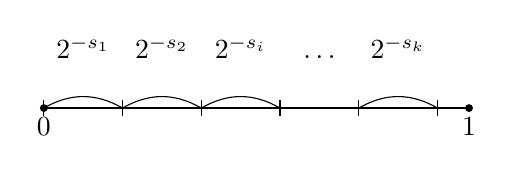
\begin{tikzpicture}          
        \draw[-, thick] (0,0) -- (5.4,0);           
        \foreach \x in {1,2} {
            \draw (\x-1,0.1) -- (\x-1,-0.1);
            \node[above] at (\x-0.5, 0.5) {$2^{-s_{\x}}$};
            \draw (\x-1,0) to[bend left=30] (\x,0);
        }
        \draw (2,0.1) -- (2,-0.1);
        \node[above] at (2.5, 0.5) {$2^{-s_{i}}$};
        \draw (2,0) to[bend left=30] (3,0);
        \draw (3,0.1) -- (3,-0.1);
        \node[above] at (3.5, 0.5) {$\ldots$};
        \draw (4,0.1) -- (4,-0.1);
        \node[above] at (4.5, 0.5) {$2^{-s_{k}}$};
        \draw (5,0.1) -- (5,-0.1);
        \draw (4,0) to[bend left=30] (5,0);
        \fill[black] (0,0) circle (0.05) node[below] {0};
        \fill[black] (5.4,0) circle (0.05) node[below] {1};
    \end{tikzpicture}\\
    Утверждение: $\frac{1}{2}$ является границей отрезков. (не может лежать внутри какого либо $2^{-s_i}$)\\
    Предположим, что это не так, тогда:

    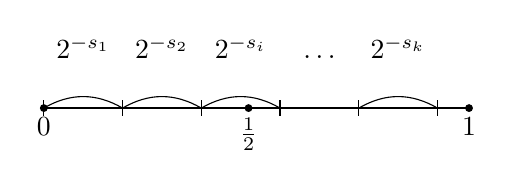
\begin{tikzpicture}          
        \draw[-, thick] (0,0) -- (5.4,0);           
        \foreach \x in {1,2} {
            \draw (\x-1,0.1) -- (\x-1,-0.1);
        
            \node[above] at (\x-0.5, 0.5) {$2^{-s_{\x}}$};
            \draw (\x-1,0) to[bend left=30] (\x,0);
        }
        \draw (2,0.1) -- (2,-0.1);
        \node[above] at (2.5, 0.5) {$2^{-s_{i}}$};
        \draw (2,0) to[bend left=30] (3,0);
        \draw (3,0.1) -- (3,-0.1);
        \node[above] at (3.5, 0.5) {$\ldots$};
        \draw (4,0.1) -- (4,-0.1);
        \node[above] at (4.5, 0.5) {$2^{-s_{k}}$};
        \draw (5,0.1) -- (5,-0.1);
        \draw (4,0) to[bend left=30] (5,0);
        \fill[black] (2.6,0) circle (0.05) node[below] {$\frac{1}{2}$};
        \fill[black] (0,0) circle (0.05) node[below] {0};
        \fill[black] (5.4,0) circle (0.05) node[below] {1};
    \end{tikzpicture}\\
    Имеем неравенства:
    
    $$\begin{cases}
        2^{-s_1} + \ldots + 2^{-s_{i-1}} \leq \frac{1}{2}\\
        2^{-s_1} + \ldots + 2^{-s_{i-1}} + 2^{-s_i} > \frac{1}{2}
    \end{cases} \text{домножим на } 2^{s_{i}}\implies$$

    $$\implies \begin{cases}
        \underbrace{2^{s_i - s_1} + \ldots + 2^{s_i - s_{i-1}}}_c < 2^{s_i-1}\\
        \underbrace{2^{s_i - s_1} + \ldots + 2^{s_i - s_{i-1}}}_c + 1 > 2^{s_i-1}
    \end{cases} \implies \begin{cases}
        c < 2^{s_i-1}\\
        c + 1 > 2^{s_i-1}
    \end{cases} \text{ --- противоречие.}$$\\
    Таким образом какой-то отрезок из $2^{-s_i}$ упрется в $\frac{1}{2}$ или хотя бы не дойдет до нее. Тогда 
    Разделим $2^{-s_1}, 2^{-s_2}, \ldots, 2^{-s_k}$ на 2 части: те, которые меньше $\frac{1}{2}$ и те, которые больше.
    Тем кодам, которые меньше $\frac{1}{2}$ поставим 0 в начало кода, а тем, которые больше $\frac{1}{2}$ поставим 1, тогда их длина уменьшилась на единицу. 
    Тогда сумма тех, что слева и тех, что справа:
    \[\sum 2^{-(s_i-1)} = \sum 2 \cdot 2^{-s_i} = 2 \cdot \sum 2^{-s_i} \leq 1\]
    Тогда можем рекурсивно выполнять деление отрезков, т.к. если есть всего 2 символа,
    можем дать им коды 0 и 1 соответственно.
\end{proof}

\section{Задача о наилучших длинах кодов}
Пусть $A = \{c_1, \ldots, c_n\}$ --- алфавит, $p_1, \ldots, p_n$ --- вероятности появления символов. Пусть задан код $\phi: A \to \{0, 1\}^*$\\
Фиксируем текст (большую строку) длины $N: a_1 a_2\ldots a_N$. В этом тексте количество символов $c_i$ -- $N \cdot a_i$ (закон больших чисел). Тогда длина кодовой последовательности текста:

\[\sum_{i=1}^{n} N p_i \phi(c_i)\]
Задача заключается в том, чтобы минимализировать длину кодовой последовательности такого текста,
а т.к. $N$ -- фиксированная величина, не влияющая на коды, задача сводиться к тому, чтобы минимализировать сумму:
\[\sum_{i=1}^{n}p_i \phi(c_i)\]
При этом для $p_i, \phi(c_i)$ выполняются:
\begin{enumerate}
    \item $\sum p_i = 1$
    \item $0 < p_i < 1$
    \item $\phi(c_i) > 0, \phi(c_i) \in \Z$
    \item $\phi(c_1), \ldots, \phi(c_n)$ -- длины кодов символов в префиксом коде, т.е. для этих длин выполняется неравенство Крафта.
\end{enumerate}

\begin{remark}
    По правде говоря, из приведенного доказательства неравенства Крафта 
    не следует, что код будет префиксным, но это можно вывести. Кто-нибудь умный скажет,
    как это сделать.
\end{remark}

\begin{theorem}
    Минимум достигается функцией:
    \[H(p) = \sum_{i=1}^{n} \log_{2} \frac{1}{p_i} \label{eq:entropy}\]
\end{theorem}

% TODO
\begin{proof}
    
\end{proof}

\section{Энтропия}
\begin{definition}
    Энтропией вероятностной схемы называется мера содержащейся в ней 
    неопределенности. Она задается как конкретная функция $H: RS \to \R^+$, где $RS$ -- множество всех возможных вероятностных схем. 
\end{definition}
Функция, задающая энтропию обладает рядом свойств, и этим свойствам удовлетворяет
функция $\ref{eq:entropy}$. Это докажем позже, а сейчас рассмотрим свойства энтропии: 

\begin{properties}
    $\newline$
    \begin{enumerate}
        \item Мера неопределенности непрерывно зависит от вероятностей. 
        (функция $\ref{eq:entropy}$ этим свойством, очевидно, обладает)
        \item При перестановке вероятностей мера неопределенности не меняется.
        \item Необходимо ввести единицу измерения неопределенности. За единицу будем
        брать энтропию честной монеты: $H(\{\frac{1}{2}, \frac{1}{2}\}) = 1$ -- бит.
        \item Обозначим за $h(m) = H(\{\frac{1}{m}, \frac{1}{m}, \ldots, \frac{1}{m}\})$. Тогда $h(m)$ растет с ростом $m$. 
        (функция $\ref{eq:entropy}$ этим свойством тоже обладает)
        \item При фиксированном $m$ максимум энтропии достигается в случае равновероятных исходов, т.е. $h(m)$.
        \item Пусть есть схемы $P_m = p_1, \ldots, p_m$ и $Q_k = q_1, \ldots, q_k$. Образуем комбинированную схему с 
        $m - k + 1$ исходами следующим образом: выбирается $m$-й исход в $P_m$ и для него выбираются исходы из $Q_k$. Получим 
        схему $PQ$ с ихсодами: $$1, 2, \ldots, m-1, (m, 1), (m, 2), \ldots, (m, k)$$
        Вероятность этих исходов: $$p_1, \ldots, p_{m-1}, p_m q_1, \ldots, p_m q_k$$
        Тогда энтропия схемы $PQ: H(PQ) = H(P_k) + p_m H(Q_k)$
    \end{enumerate}
\end{properties}

\begin{proof} (Какие-то свойства либо уже доказаны, либо были даны без доказательства)
    \begin{enumerate}
        \item[6]
        \[H(PQ) = \sum_{i=1}^{m-1}p_i \log_2 \frac{1}{p_i} + \sum_{j=1}^{k} p_m q_j \log_2 \frac{1}{p_m q_j} =\]
        \[= \sum_{i=1}^{m-1}p_i \log_2 \frac{1}{p_i} + p_m \sum_{j=1}^{k}q_j \log_2 \frac{1}{p_m} + p_m \sum_{j=1}^{k}q_j \log_2 \frac{1}{q_j} = \]
        \[= 1 \cdot p_m \log_2 \frac{1}{p_m} +  \sum_{i=1}^{m-1}p_i \log_2 \frac{1}{p_i} + p_m \sum_{j=1}^{k}q_j \log_2 \frac{1}{q_j} = H(P_m) + p_m H(Q_k)\]
    \end{enumerate}
\end{proof}